\subsection{Configurazione Database}
Si è optato per l'utilizzo di \textit{ClickHouse} per il salvataggio dei dati, le motivazioni sono descritte nella sezione \ref{sec:clickHouse}. In particolare, per ogni sensore dei quali si desidera memorizzare i dati, viene creata una tabella che acquisisce i dati dal relativo topic Kafka.
Le tipologie di sensori cui misurazioni si vogliono trattare nel progetto sono:
\begin{itemize}
    \item Sensori di temperatura;
    \item Sensori di umidità;
    \item Sensori stato riempimento isole ecologiche;
    \item Sensori di stato occupazione colonnine di ricarica;
    \item Sensori di guasti elettrici;
    \item Sensori del livello dell'acqua.
\end{itemize}

La configurazione del database \textit{ClickHouse} è stata un elemento fondamentale nella progettazione, poiché un'adeguata impostazione consente prestazioni adeguate per un sistema orientato al tempo reale e in grado di gestire analisi su enormi quantità di dati.

\subsubsection{Funzionalità Clickhouse utilizzate}
\paragraph{Materialized Views}
Le Materialized Views in \textit{ClickHouse} sono un meccanismo potente per migliorare le prestazioni delle \textit{Query} e semplificare l'accesso ai dati. Funzionano mantenendo una copia fisica dei risultati di una \textit{Query} di selezione, che viene quindi memorizzata su disco. Questa copia è aggiornata periodicamente in base ai dati sottostanti.

\paragraph*{Utilizzi Principali}
\begin{itemize}
    \item \textbf{Calcolo aggregazioni e popolamento tabelle}:Spesso le delle materialized Views sono state utilizzate per calcolare aggregazioni su dati e quindi popolare altre tabelle con i risultati aggregati. Ad esempio, nel caso specifico in cui una Materialized View calcola la media delle temperature per ogni sensore ogni secondo, i risultati di questa vista possono essere utilizzati per popolare una tabella principale contenente i dati di temperatura aggregati, aggiornando i valori di temperatura medi per ogni sensore ogni secondo;
    \item \textbf{Ottimizzazione delle Prestazioni}: memorizzando i risultati di una \textit{Query} complessa, le Materialized Views consentono di eseguire rapidamente le \textit{Query} successive senza dover ricalcolare i dati ogni volta. Ciò è particolarmente utile in applicazioni che richiedono interrogazioni frequenti su grandi volumi di dati;
    \item \textbf{Aggregazioni Pre-Calcolate}: le Materialized Views possono essere utilizzate per pre-calcolare aggregazioni, come somme, medie o conteggi, sui dati sottostanti. Questo può migliorare notevolmente le prestazioni delle \textit{Query} che coinvolgono operazioni di aggregazione;
    \item \textbf{Decomposizione delle \textit{Query} Complesse}: le Materialized Views consentono di decomporre \textit{Query} complesse in passaggi più semplici e riutilizzabili, migliorando la leggibilità del codice e semplificando lo sviluppo e la manutenzione delle \textit{Query}.
\end{itemize}


\paragraph{Funzione di aggregazione avgState}
In \textit{ClickHouse}, avgState è una funzione di stato utilizzata all'interno di funzioni di aggregazione, come AggregateFunction, per calcolare la media dei valori durante l'elaborazione dei dati. Quando si utilizza avgState, ClickHouse mantiene lo stato intermedio necessario per calcolare la media dei valori inseriti. Questo stato intermedio include la somma cumulativa dei valori e il numero totale di valori inseriti.

\paragraph{AggregatingMergeTree Engine} \label{sec:AggregatingMergeTree}
Link alla documentazione: \href{https://clickhouse.com/docs/en/engines/table-engines/mergetree-family/aggregatingmergetree}{https://clickhouse.com/docs/en/engines/table-engines/mergetree-family/aggregatingmergetree}.\newline
 Specificando questo motore su di una tabella Clickhouse, vengono sostituite tutte le righe con la stessa chiave primaria (o, più accuratamente, con la stessa chiave di ordinamento) con una singola riga all'interno di una parte di dati.
 Le tabelle AggregatingMergeTree sono utilizzate per l'aggregazione incrementale dei dati, inclusa la creazione di viste materializzate aggregate.
 I campi definiti con i seguenti tipi vengono incrementale elaborati.

\paragraph{AggregateFunction}
Link alla documentazione: \href{https://clickhouse.com/docs/en/sql-reference/data-types/aggregatefunction}{https://clickhouse.com/docs/en/sql-reference/data-types/aggregatefunction}.\newline
Specifica un dato cui valore viene calcolato da una specifica funzione di aggregazione: 
\begin{verbatim}
    AggregateFunction(name, types_of_arguments…) 
\end{verbatim}
Una pratica comune per creare lo stato di una funzione di aggregazione è invocare la funzione di aggregazione aggiungendo il suffisso `-State` (ad esempio `avgState`). Per ottenere il risultato finale dell'aggregazione in un momento successivo, è essenziale utilizzare la medesima funzione di aggregazione, ma con l'aggiunta del suffisso `-Merge` (ad esempio `avgMerge` al momento della "select" del valore).
\paragraph{SimpleAggregateFunction}
Link alla documentazione: \href{https://clickhouse.com/docs/en/sql-reference/data-types/simpleaggregatefunction}{https://clickhouse.com/docs/en/sql-reference/data-types/simpleaggregatefunction}.\newline
Il tipo di dato:
\begin{verbatim}
    SimpleAggregateFunction(name, types_of_arguments...)
\end{verbatim}  memorizza il valore attuale della funzione di aggregazione, senza conservare l'intero stato come fa AggregateFunction.
I valori del tipo di dato SimpleAggregateFunction(func, Type) vengono visualizzati e memorizzati nello stesso modo di Type, pertanto non è necessario applicare le funzioni con suffissi -Merge/-State.

SimpleAggregateFunction offre prestazioni migliori rispetto a AggregateFunction con la stessa funzione di aggregazione ma non sono disponibili tutte le tipoligie di funzioni di aggregazione come il calcolo della media.


    
\paragraph{Projection}\label{sec:projections}
Link alla documentazione: \href{https://clickhouse.com/docs/en/sql-reference/statements/alter/projection}{https://clickhouse.com/docs/en/sql-reference/statements/alter/projection}\newline
Le proiezioni memorizzano i dati in un formato che ottimizza l'esecuzione delle \textit{Query}, questa caratteristica è utile per:

\begin{itemize}
    \item Eseguire \textit{Query} su una colonna che non fa parte della chiave primaria;
    \item Pre-aggregare colonne, riducendo sia i calcoli che l'I/O.
\end{itemize}

Puoi definire una o più proiezioni per una tabella e durante l'analisi della \textit{Query} la proiezione con meno dati da esaminare sarà selezionata da ClickHouse senza modificare la \textit{Query} fornita dall'utente.

\paragraph*{Utilizzo dello spazio su disco}
\textbf{Attenzione:} le proiezioni creeranno internamente una nuova tabella nascosta, ciò significa che saranno necessari più I/O e spazio su disco. Ad esempio, se la proiezione ha definito una chiave primaria diversa, tutti i dati dalla tabella originale verranno duplicati.

\subsubsection{Tabella delle misurazioni per sensore generico}
Le tabelle del database impiegate per registrare le misurazioni di ciascuna tipologia di sensore presentano una configurazione sostanzialmente simile, differenziandosi principalmente per il tipo di dato della colonna relativa alla misurazione e per il \textit{topic} di riferimento utilizzato per ottenere le misurazioni.
Nello specifico per ogni sensore si avrà la seguente tabella Clickhouse:
\begin{figure}[H]
    \centering
    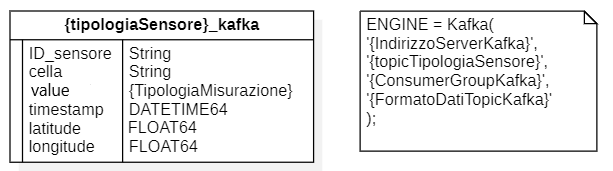
\includegraphics[width=.6\textwidth]{../Images/SpecificaTecnica/sensorType_kafka.PNG}
    \caption{Tabella sensore generico per il reperimento da kafka - ClickHouse}
    \label{fig:sensorKafka}
  \end{figure}

    La tabella è configurata con il motore di storage \textit{Kafka}, il che significa che i dati verranno letti da un \textit{topic Kafka}. 

    I campi sono:
    \begin{itemize}
        \item \textbf{ID\_sensore}: un campo di tipo \textit{String} che identifica univocamente il sensore che ha effettuato la misurazione;
        \item \textbf{cella}: un campo di tipo \textit{String} che rappresenta la cella della città in cui è stata effettuata la misurazione;
        \item \textbf{value}: un campo di tipo variabile a seconda del tipo di misurazione che contiene il valore della temperatura;
        \item \textbf{timestamp}: campo di tipo \textit{DATETIME64} che rappresenta il timestamp della misurazione della temperatura;
        \item \textbf{latitude}: un campo di tipo \textit{Float64} che rappresenta la latitudine del luogo dove è stata effettuata la misurazione;
        \item \textbf{longitude}: un campo di tipo \textit{Float64} che rappresenta la longitudine del luogo dove è stata effettuata la misurazione.
    \end{itemize}

    Mentre i parametri esposti racchiusi da parentesi graffe variano per ogni tipolgia di sensore correlato alla misurazione e sono:
    \begin{itemize}
        \item \textbf{tipologiaSensore}: viene sostituito con la tipologia del sensore che effettua le misurazioni salvate nella tabella; (ex. temperatures)
        \item \textbf{TipoDatoMisurazione}: viene sostituito con il tipo del dato che rappresenta la misurazione (ex. Float32, UInt8);
        \item \textbf{IndirizzoServerKafka}: specifica l'indirizzo del server Kafka.
        Nel nostro caso il server Kafka è in esecuzione su un container \textit{Docker} raggiungibile tramite l'indirizzo:
         \textit{'kafka:9092'};
        \item \textbf{topicTipologiaSensore}: specifica il nome del topic Kafka da cui leggere i dati (ex.temperature);
        \item \textbf{ConsumerGroupKafka}: specifica il nome del consumer group Kafka che verrà utilizzato per leggere i messaggi dal topic \textit{Kafka} denominato 'temperature'.
        Un consumer group in \textit{Kafka} è un gruppo di consumatori che lavorano insieme per consumare i messaggi da uno o più topic. Ogni messaggio inviato a un \textit{topic Kafka} può essere consumato da uno dei consumatori nel gruppo. I consumer all'interno di uno stesso gruppo condividono l'elaborazione dei messaggi all'interno dei topic: ogni messaggio viene elaborato da uno e un solo consumatore all'interno del gruppo. Nel nostro caso sarà sempre '\textit{CG\_Clickhouse\_1}' per indicare il servizio di salvataggio \textit{Clickhouse}.
        \item \textbf{FormatoDatiTopicKafka}: specifica il formato dei dati nel \textit{topic Kafka}. Nel nostro caso, i dati sono nel formato JSONEachRow, che è un formato di serializzazione JSON di \textit{ClickHouse} che consente di scrivere o leggere record JSON separati da una riga. Quindi avremo che <<FormatoDatiTopicKafka>> = JSONEachRow.
    \end{itemize}

    
\subsubsection{Misurazioni temperatura} \label{sec:tab_temperatures}
Di seguito viene fornita la configurazione riguardante il salvataggio delle misurazioni di temperatura:
\paragraph{Tabella: temperatures\_kafka}
\begin{figure}[H]
    \centering
    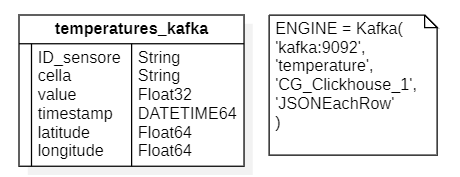
\includegraphics[width=1\textwidth]{../Images/SpecificaTecnica/temperatures_kafka.PNG}
    \caption{Tabella temperatures\_kafka - ClickHouse}
    \label{fig:temperaturesKafka}
  \end{figure}

Il dato della misurazione è di tipo Float32, l'equivalente di float nel linguaggio \textit{C}.
Il topic kafka per ottenere i dati è: \textit{temperature}.

Considerando la possibilità di ricevere molteplici misurazioni dei dati di temperatura all'interno di un singolo secondo di tempo, si procede alla creazione della seguente tabella e alla materialized view correlata, il cui obiettivo è aggregare le misurazioni di temperatura per ridurle ad una singola misurazione per secondo.

\paragraph{Tabella: temperatures}
\begin{figure}[H]
    \centering
    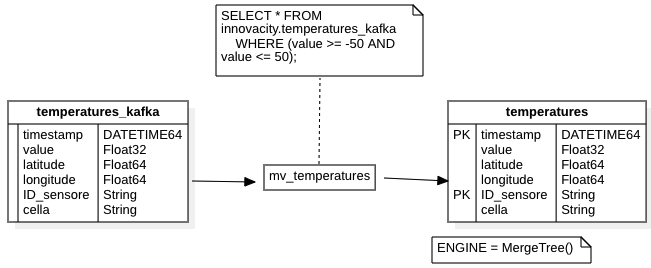
\includegraphics[width=1\textwidth]{../Images/SpecificaTecnica/temperatures.PNG}
    \caption{Tabella temperatures - ClickHouse}
    \label{fig:temperatures}
  \end{figure}

    Nello specifico la MATERIALIZED VIEW \textit{mv\_temperatures} ottiene i dati dalla tabella dei dati raccolti dal topic kafka,calcola la media dei delle misurazioni all'interno dello stesso secondo e le salva nella tabella \textit{temperatures}.
    Questa tramite il motore \textit{AggregatingMergeTree}, cui funzione viene definita in \ref*{sec:AggregatingMergeTree}, calcola incrementalmente la media delle misurazioni nel secondo.

    Lo stesso viene fatto per ottenere delle tabelle con i valori delle misurazioni aggregati tramite media per ottenere un dato per: minuto, ora, giorno e mese.
    Le tabelle risultanti sono denominatate: \textbf{temperatures1m, temperatures1o, temperatures1g e temperatures1M}. Queste tabelle presentano la stessa struttura della tabella originale, differenziandosi solo per il tipo di dato del campo timestamp, che rispettivamente è: \textbf{DateTime, DateTime, Date32 e Date32}, per la funzione utilizzata per calcolare il campo timestamp, che sono rispettivamente: \textbf{toStartOfMinute, toStartOfHour, toDate e toStartOfMonth} e perchè non contengono i campi : \textbf{latitude} e \textbf{longitude}.
    Il ragionamento alla base di questa decisione è che la posizione geografica del sensore è rilevante solo nella tabella delle aggregazioni per secondo. Questa tabella è utilizzata da servizi come \textit{Grafana} per recuperare e visualizzare l'ultima posizione del sensore su una mappa. D'altro canto, le tabelle con aggregazioni su periodi temporali più ampi (come minuti, ore, ecc.) non hanno bisogno di salvare la posizione del sensore, poiché sono utilizzate esclusivamente per analizzare il valore aggregato delle misurazioni.
    In sintesi nelle tabelle che aggregano le misurazioni per minuto, ora o giorno, la posizione specifica del sensore in un dato istante diventa meno rilevante poiché queste tabelle rappresentano aggregazioni su periodi più lunghi. In queste situazioni, l'obiettivo principale è analizzare i valori aggregati delle misurazioni nel tempo. 

    \paragraph{Tabella: temperatures1m}
    \begin{figure}[H]
        \centering
        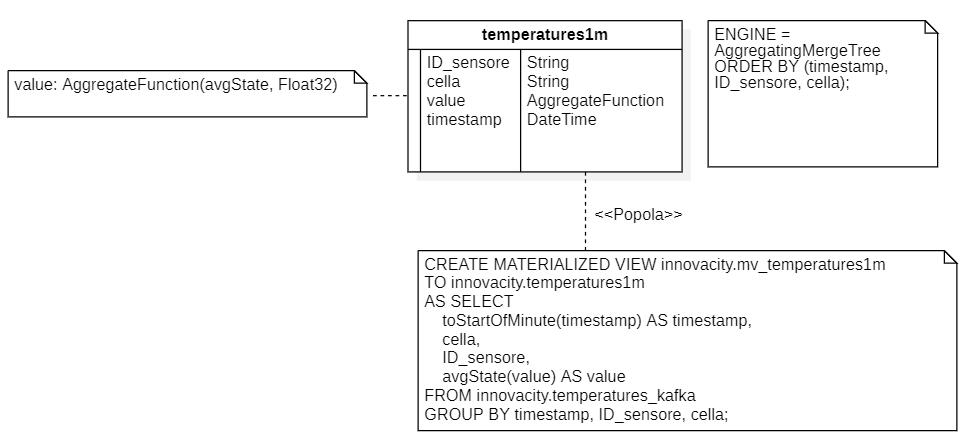
\includegraphics[width=1\textwidth]{../Images/SpecificaTecnica/temperatures1m.PNG}
        \caption{Tabella temperatures1m - ClickHouse}
        \label{fig:temperatures1m}
      \end{figure}
      \paragraph{Tabella: temperatures1o}
      \begin{figure}[H]
          \centering
          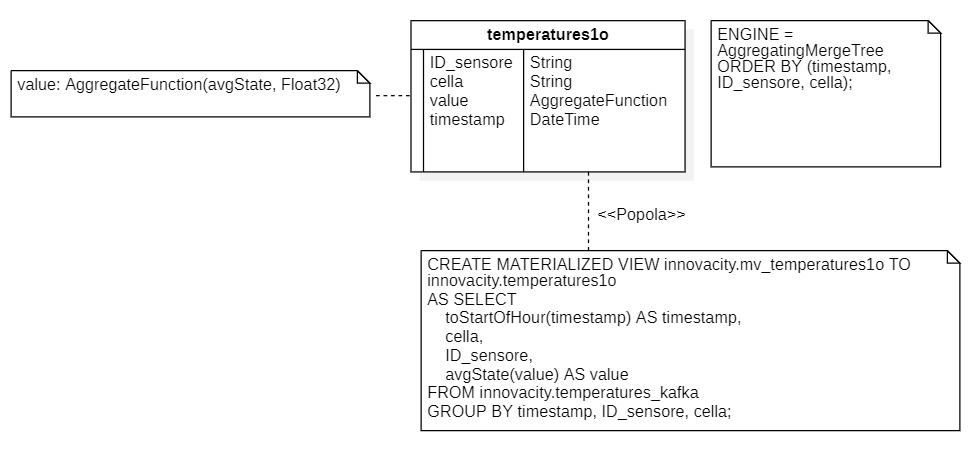
\includegraphics[width=1\textwidth]{../Images/SpecificaTecnica/temperatures1o.PNG}
          \caption{Tabella temperatures1o - ClickHouse}
          \label{fig:temperatures1o}
        \end{figure}
    \paragraph{Tabella: temperatures1g}
    \begin{figure}[H]
        \centering
        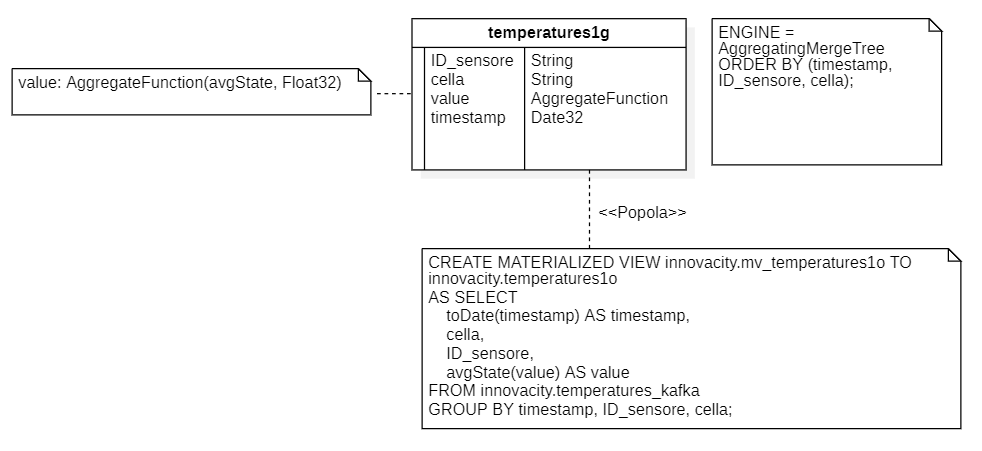
\includegraphics[width=1\textwidth]{../Images/SpecificaTecnica/temperatures1g.PNG}
        \caption{Tabella temperatures1g - ClickHouse}
        \label{fig:temperatures1g}
        \end{figure}
    \paragraph{Tabella: temperatures1M}
    \begin{figure}[H]
        \centering
        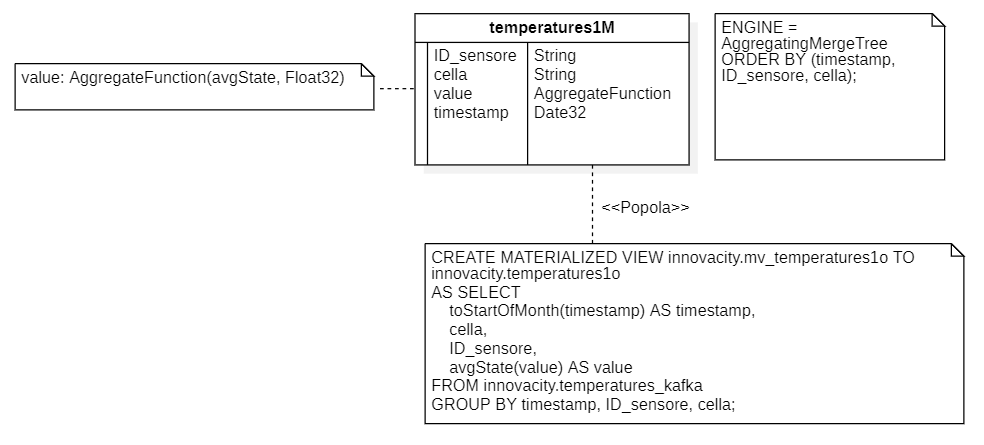
\includegraphics[width=1\textwidth]{../Images/SpecificaTecnica/temperatures1Mese.PNG}
        \caption{Tabella temperatures1M - ClickHouse}
        \label{fig:temperatures1M}
        \end{figure}
    
    \paragraph{Projections per misurazioni di temperatura} \label{sec:temp_projections}
    Durante la fase di progettazione, è stata posta particolare attenzione all'utilizzo delle tabelle appena descritte e alle richieste che verranno formulate su di esse. È emerso che saranno frequenti le \textit{Query} che filtrano le misurazioni in base a due date specifiche.
    In aggiunta, considerando il requisito di suddividere la città in una serie di celle e specificare la cella di origine della misurazione, la filtrazione delle misurazioni per celle diventerà una richiesta effettuata con frequenza al database.
    Si è giunti quindi all'utilizzo delle \textit{PROJECTIONS}, descritte nella sezione \ref{sec:projections}.

    \begin{lstlisting}
        --Projection per tabella temperatures
        ALTER TABLE innovacity.temperatures ADD PROJECTION sensor_cell_projection (SELECT * ORDER BY cella, timestamp);
        ALTER TABLE innovacity.temperatures MATERIALIZE PROJECTION sensor_cell_projection;
    \end{lstlisting}

    La proiezione ci permetterà di filtrare per \textit{cella} e \textit{timestamp} rapidamente, anche se nella tabella originale queste non sOno definite come \textit{PRIMARY\_KEY}.

    Vengono create delle \textit{PROJECTIONS} anche per le tabelle:  \textbf{temperatures1m, temperatures1o, temperatures1g}
    ma non per  \textbf{temperatures1M} in quanto anche a lungo andare la quantità di dati presente in essa non sarà massiva.

    \begin{lstlisting}
        --Projection per tabella temperatures1m
        ALTER TABLE innovacity.temperatures1m ADD PROJECTION sensor_cell_projection1m (SELECT * ORDER BY cella,timestamp);
        ALTER TABLE innovacity.temperatures1m MATERIALIZE PROJECTION sensor_cell_projection1m;

        --Projection per tabella temperatures1o
        ALTER TABLE innovacity.temperatures1o ADD PROJECTION sensor_cell_projection1o (SELECT * ORDER BY cella,timestamp);
        ALTER TABLE innovacity.temperatures1o MATERIALIZE PROJECTION sensor_cell_projection1o;

        --Projection per tabella temperatures1g
        ALTER TABLE innovacity.temperatures1g ADD PROJECTION sensor_cell_projection1g (SELECT * ORDER BY cella,timestamp);
        ALTER TABLE innovacity.temperatures1g MATERIALIZE PROJECTION sensor_cell_projection1g;
    \end{lstlisting}

    \paragraph{Analisi benefici delle Projections}\label{sec:temp_projections_benefici}
    L'aggiunta delle \textit{PROJECTIONS} ha portato risultati di estremo rilievo di seguito esposti.
    Prendendo una \textit{Query} tipo svolta per l'analisi da \textit{Grafana}:
    \begin{figure}[H]
        \centering
        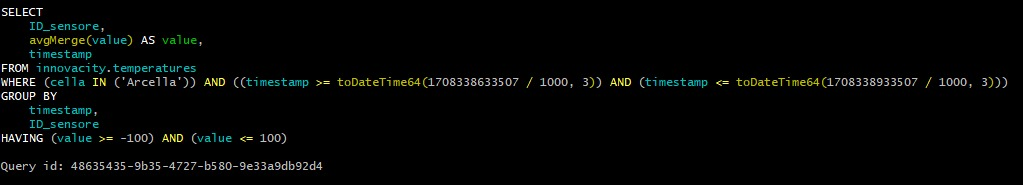
\includegraphics[width=1\textwidth]{../Images/SpecificaTecnica/ProjectionQuery.jpg}
        \caption{Query tipica - Grafana}
        \label{fig:ProjectionsQuery}
      \end{figure}
    senza l'utilizzo delle \textit{PROJECTIONS} il risultato è:
    \begin{figure}[H]
        \centering
        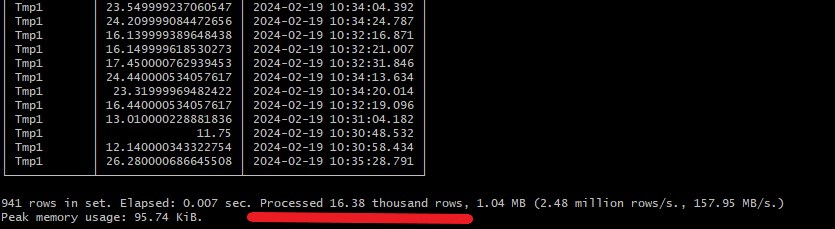
\includegraphics[width=0.9\textwidth]{../Images/SpecificaTecnica/SenzaProectionResult.jpg}
        \caption{Query tipica risultato senza projections}
        \label{fig:ProjectionsQueryWthout}
      \end{figure}
      ovvero sono state processate per ottenere il risultato della \textit{Query} 16,38 migliaia di righe.

      Invece in seguito all'aggiunta delle \textit{PROJECTIONS}:
      \begin{figure}[H]
        \centering
        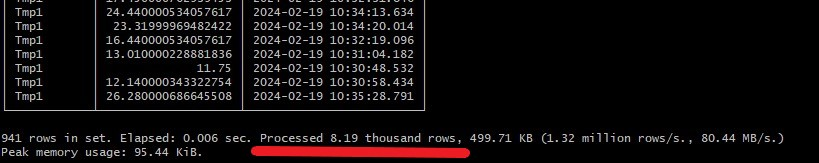
\includegraphics[width=0.9\textwidth]{../Images/SpecificaTecnica/ConProjectionRisultato.jpg}
        \caption{Query tipica risultato con projections}
        \label{fig:ProjectionsQueryWith}
      \end{figure}   
  ovvero sono state processate per ottenere il risultato della \textit{Query} 8,19 migliaia di righe, circa la metà rispetto al risultato precedente consentendoci di apprezzare il miglioramento.
Inoltre tramite una \textit{Query} speciale è possibile visualizzare che la \textit{PROJECTIONS} è stata effettivamente utilizzata per ottenere il risultato della \textit{Query} in esame.
\begin{figure}[H]
    \centering
    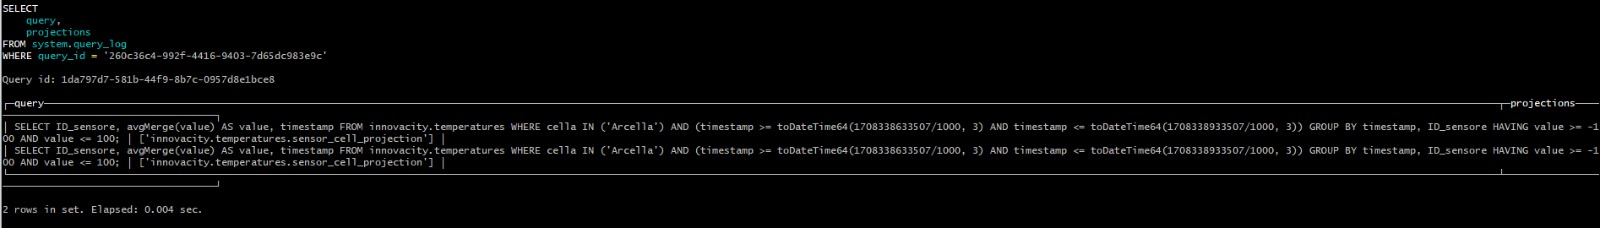
\includegraphics[width=1\textwidth]{../Images/SpecificaTecnica/ProjectionUsedByClickHouse.jpg}
    \caption{Uso della Projection}
    \label{fig:ProjectionsUsed}
\end{figure}

\subsubsection{Misurazioni umidità}
Le considerazioni relative al salvataggio delle misurazioni di umidità coincidono con quelle espresse nella sezione \ref{sec:tab_temperatures} riguardo alle misurazioni di temperatura.
\paragraph{Tabella: umidities\_kafka}
\begin{figure}[H]
    \centering
    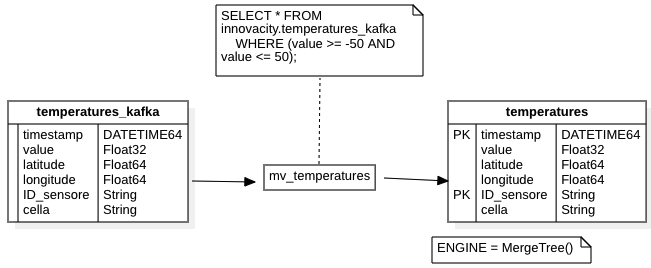
\includegraphics[width=1\textwidth]{../Images/SpecificaTecnica/temperatures.PNG}
    \caption{Tabella umidities\_kafka - ClickHouse}
    \label{fig:umidities_kafka}
  \end{figure}
Il dato della misurazione è di tipo Float32, l’equivalente di float nel linguaggio C. Il topic
kafka per ottenere i dati è: \textbf{umidity}.
\paragraph{Tabella: umidities}
\begin{figure}[H]
    \centering
    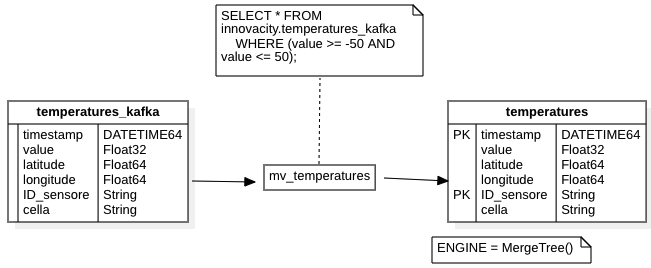
\includegraphics[width=1\textwidth]{../Images/SpecificaTecnica/temperatures.PNG}
    \caption{Tabella umidities - ClickHouse}
    \label{fig:umidities}
  \end{figure}
\paragraph{Tabella: umidities1m}
    \begin{figure}[H]
        \centering
        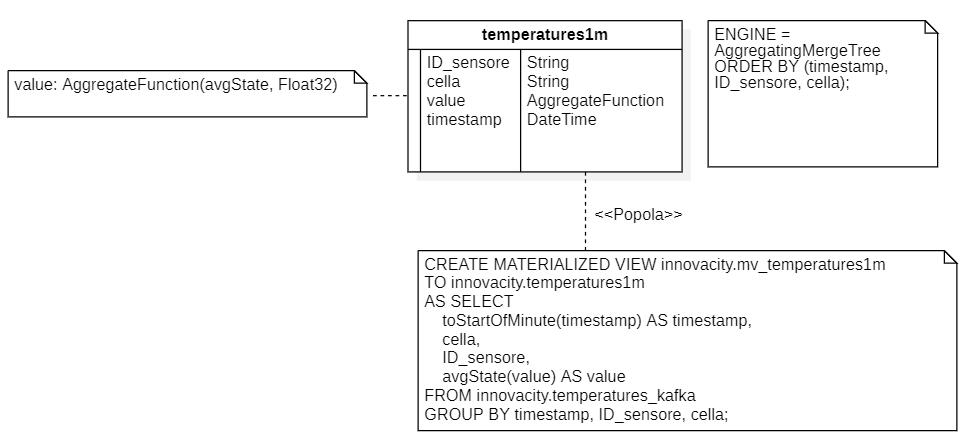
\includegraphics[width=1\textwidth]{../Images/SpecificaTecnica/temperatures1m.PNG}
        \caption{Tabella  umidities1m - ClickHouse}
        \label{fig: umidities1m}
      \end{figure}
      \paragraph{Tabella:  umidities1o}
      \begin{figure}[H]
          \centering
          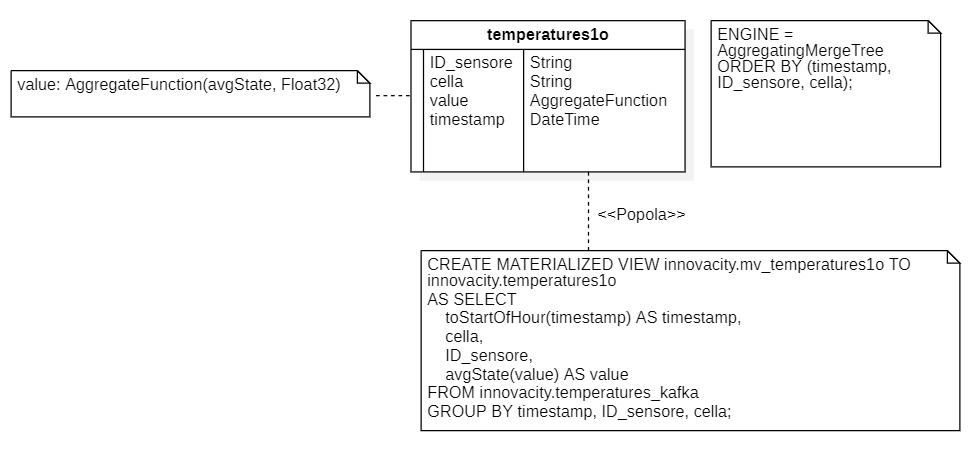
\includegraphics[width=1\textwidth]{../Images/SpecificaTecnica/temperatures1o.PNG}
          \caption{Tabella  umidities1o - ClickHouse}
          \label{fig: umidities1o}
        \end{figure}
    \paragraph{Tabella:  umidities1g}
    \begin{figure}[H]
        \centering
        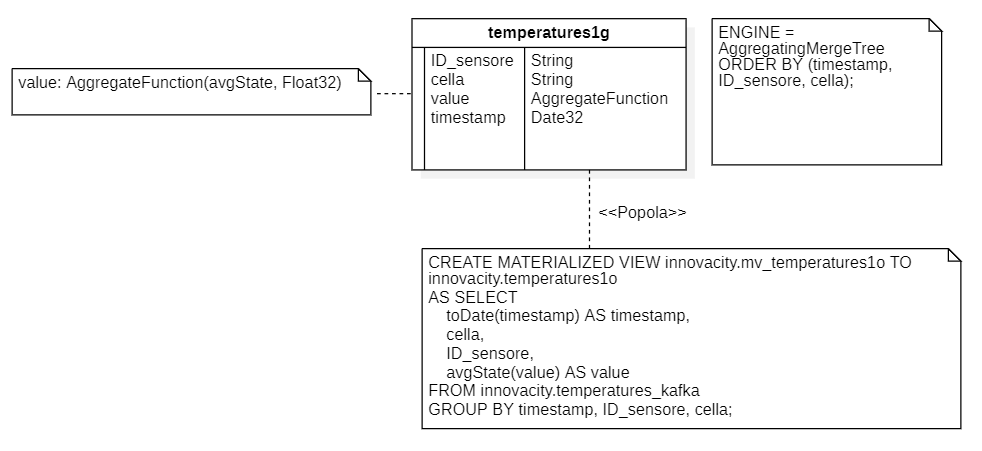
\includegraphics[width=1\textwidth]{../Images/SpecificaTecnica/temperatures1g.PNG}
        \caption{Tabella  umidities1g - ClickHouse}
        \label{fig: umidities1g}
        \end{figure}
    \paragraph{Tabella:  umidities1M}
    \begin{figure}[H]
        \centering
        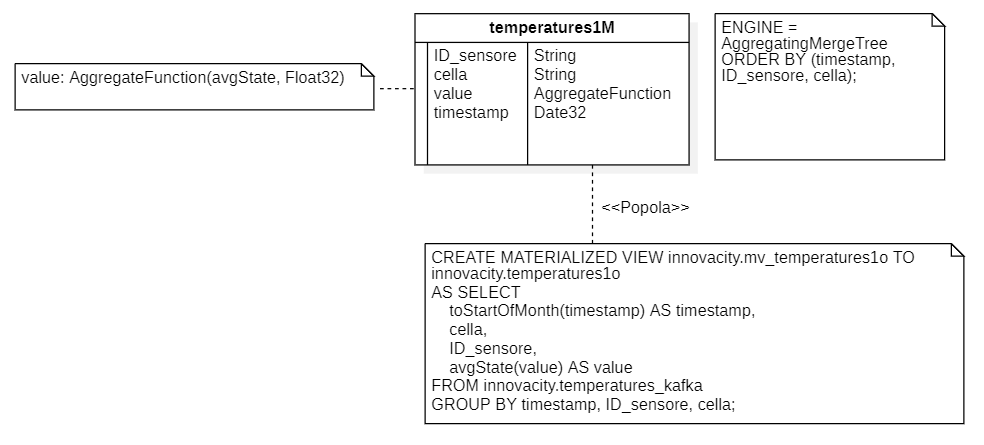
\includegraphics[width=1\textwidth]{../Images/SpecificaTecnica/temperatures1Mese.PNG}
        \caption{Tabella  umidities1M - ClickHouse}
        \label{fig: umidities1M}
        \end{figure}
\paragraph{Projections per misurazioni di umidità} 
Date le stesse considerazioni fatte nella sezione: \ref{sec:temp_projections} anche per le misurazioni di umidità si è deciso di adottare le \textit{PROJECTION}.
I risultati dei benifiici perfettamente riconducibili a quelli per le misurazioni di temperatura alla sezione: \ref{sec:temp_projections_benefici}.

Di seguito vengono fornite le configurazioni delle proiezioni sulle tabelle delle misurazioni di umidità:

\begin{lstlisting}
    --Projection per tabella umidities
    ALTER TABLE innovacity.umidities ADD PROJECTION sensor_cell_projection (SELECT * ORDER BY cella,timestamp);
    ALTER TABLE innovacity.umidities MATERIALIZE PROJECTION sensor_cell_projection;

    --Projection per tabella umidities1m
    ALTER TABLE innovacity.umidities1m ADD PROJECTION sensor_cell_projection1m (SELECT * ORDER BY cella,timestamp);
    ALTER TABLE innovacity.umidities1m MATERIALIZE PROJECTION sensor_cell_projection1m;

    --Projection per tabella umidities1o
    ALTER TABLE innovacity.umidities1o ADD PROJECTION sensor_cell_projection1o (SELECT * ORDER BY cella,timestamp);
    ALTER TABLE innovacity.umidities1o MATERIALIZE PROJECTION sensor_cell_projection1o;

    --Projection per tabella umidities1g
    ALTER TABLE innovacity.umidities1g ADD PROJECTION sensor_cell_projection1g (SELECT * ORDER BY cella,timestamp);
    ALTER TABLE innovacity.umidities1g MATERIALIZE PROJECTION sensor_cell_projection1g;
\end{lstlisting}